% Ubah judul dan label berikut sesuai dengan yang diinginkan.
\section{Desain dan Implementasi}
\label{sec:desaindanimplementasi}

\begin{enumerate}[label=\Alph*.]
    \item Diagram Blok Sistem
    \label{subsec:diagrambloksistem}

    \hspace*{1em} Sistem yang telah dirancang memiliki beberapa komponen utama, yaitu bagian sensor, bagian kontrol, bagian sistem mekanik, dan bagian \textit{motion data}. 

    \begin{figure} [h] \centering
        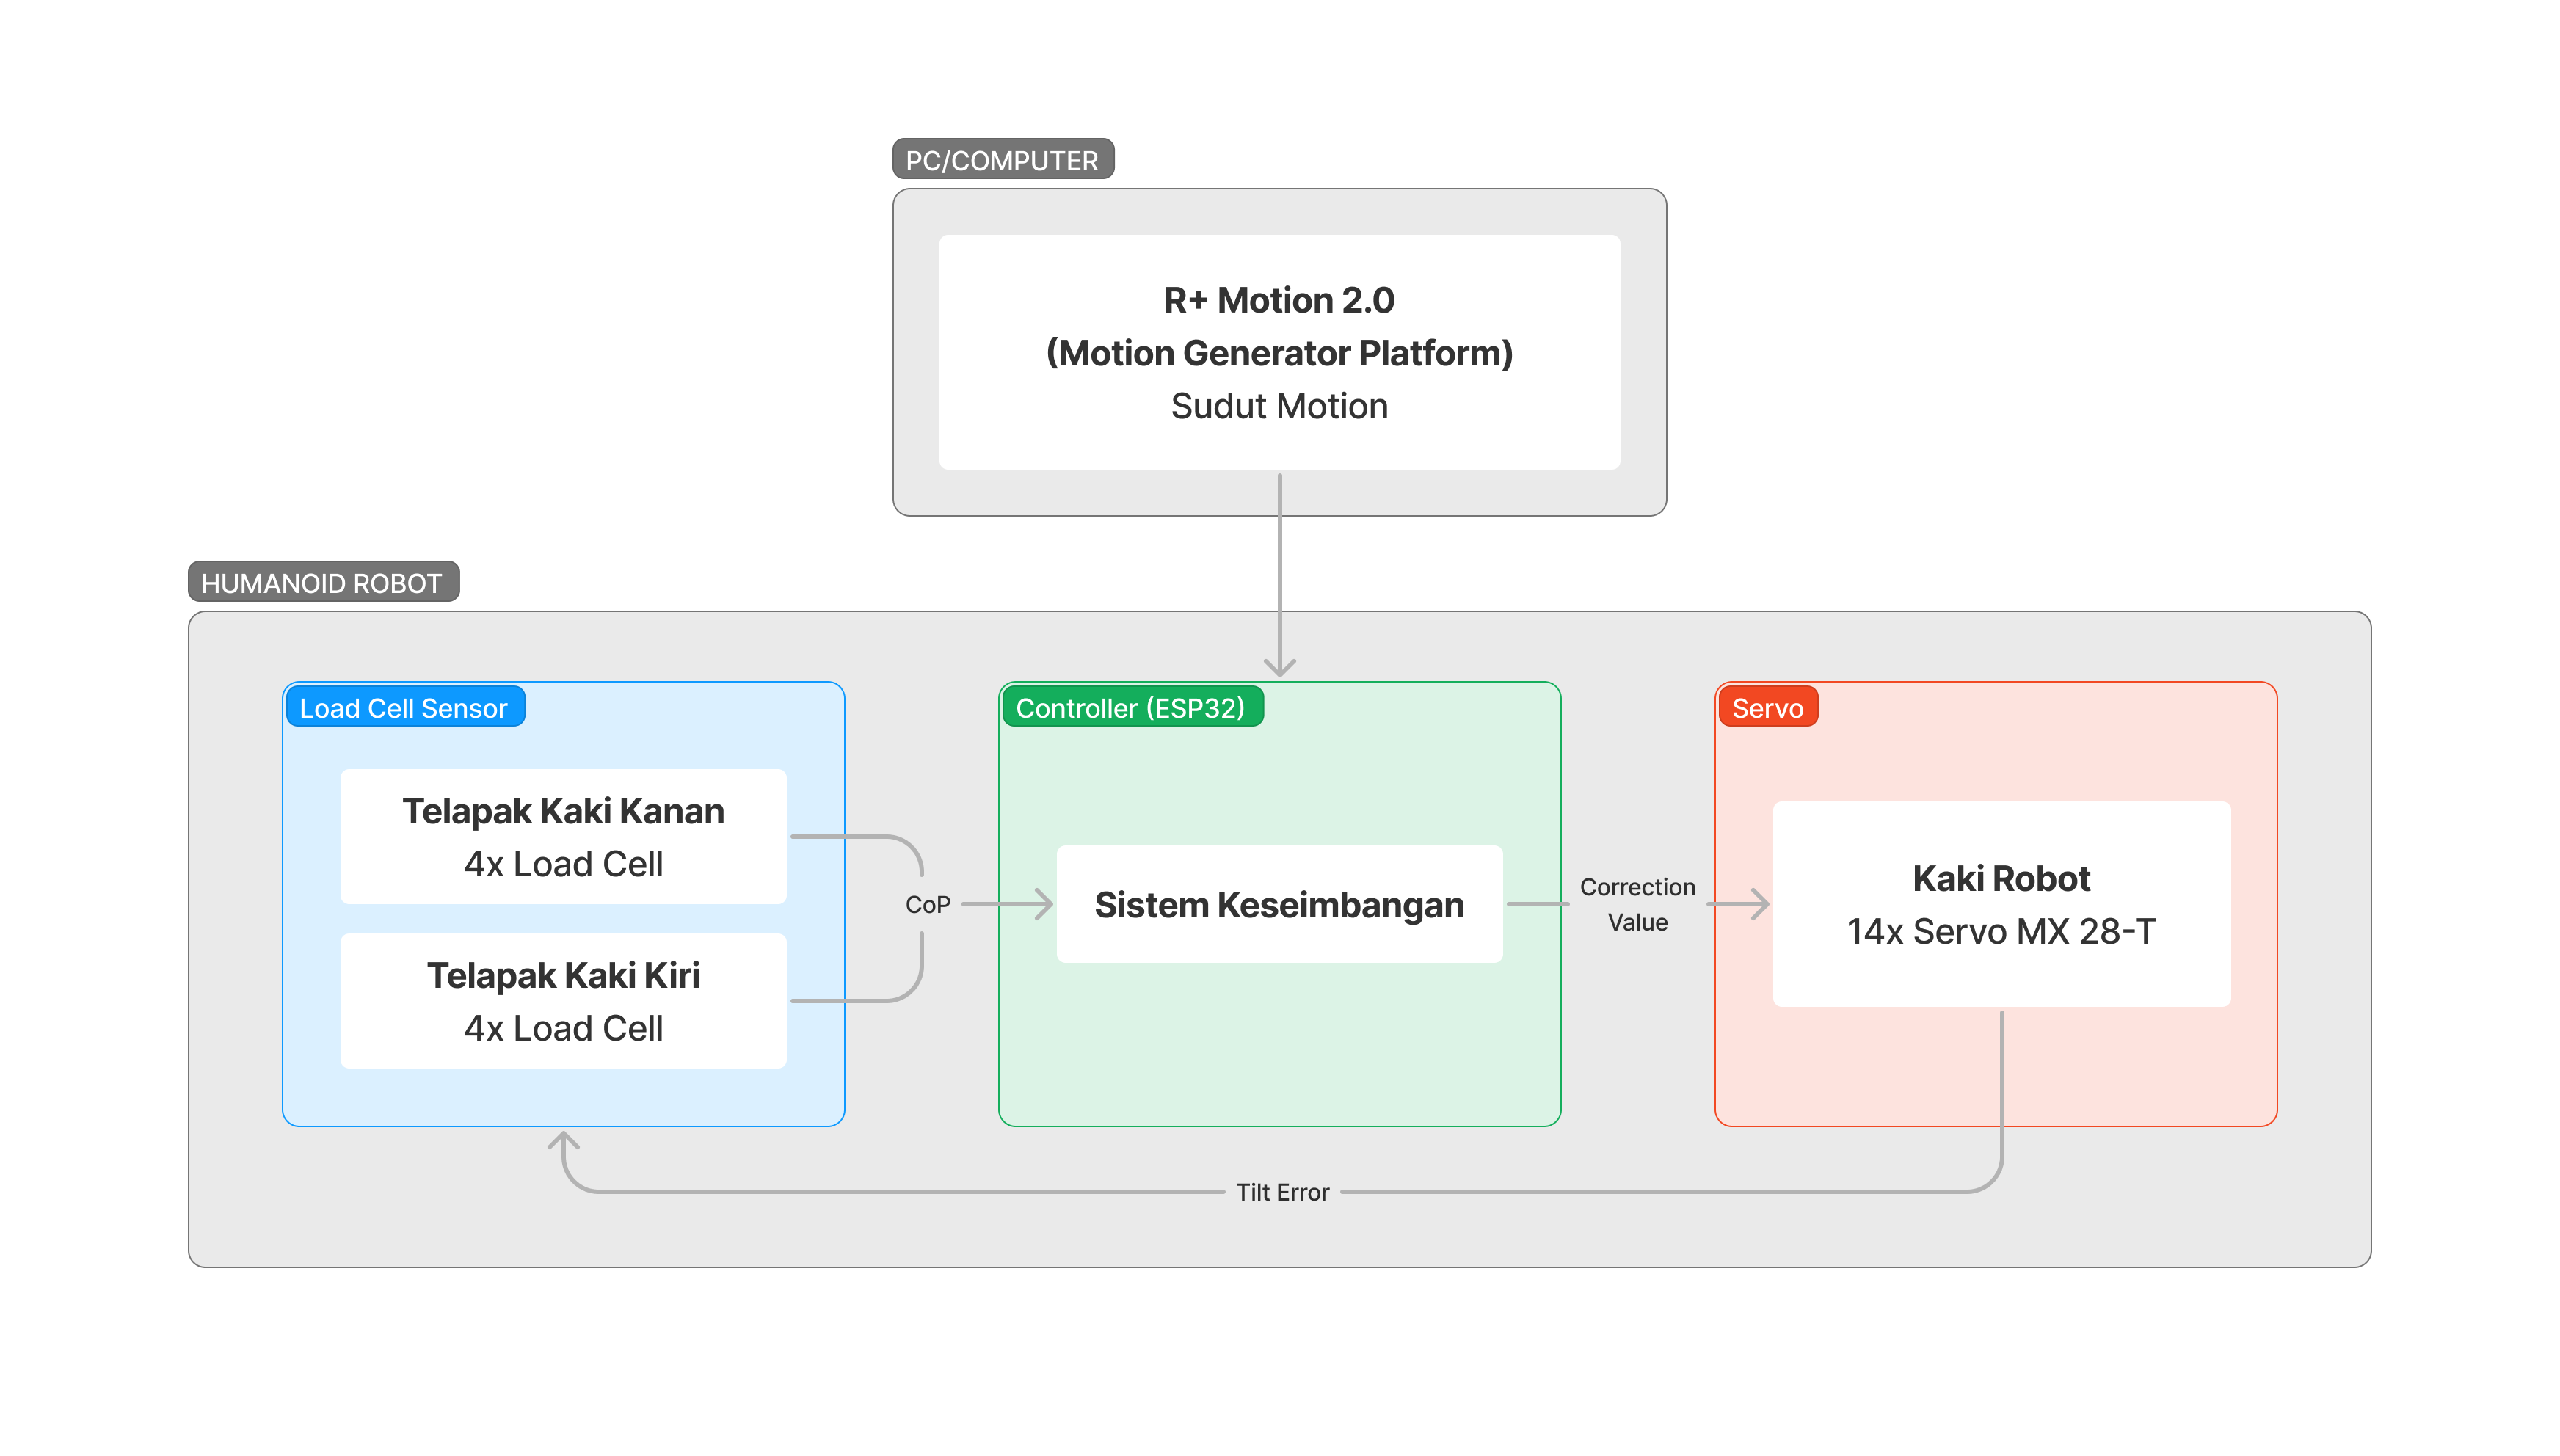
\includegraphics[width=0.45\textwidth]{gambar/Diagram_Sistem.png}
        \caption{Diagram Sistem Secara Keseluruhan}
        \label{fig:Diagram_Sistem}
    \end{figure}
    
    \hspace*{1em} Bagian sensor mencakup \emph{load cell} yang dipasang pada setiap telapak kaki robot. \emph{Load cell} ini berfungsi untuk mendeteksi beban atau tekanan pada kaki robot. Bagian kontrol melibatkan mikrokontroler yang bertanggung jawab untuk mengolah data dari sensor dan mengontrol gerakan robot. Bagian sistem mekanik mencakup kerangka robot yang terdiri dari berbagai servo yang digunakan untuk menggerakkan robot. Bagian \textit{motion data} menyimpan gerakan yang telah dirancang sebelumnya dalam sistem file mikrokontroler. Data ini terdiri dari beberapa frame yang berisi array target posisi untuk setiap servo beserta waktu yang diperlukan untuk mencapai posisi tersebut. Diagram sistem dapat dilihat pada Gambar \ref{fig:Diagram_Sistem}.
    
    \item Sistem Mekanik
    \label{subsec:sistemmekanik}

    \hspace*{1em} Desain tubuh robot humanoid ini mencakup 29 derajat kebebasan. Tubuh bagian atas menggunakan 15 servo tipe XL-320, sedangkan tubuh bagian bawah menggunakan 14 servo tipe MX-28. Rincian desain, ukuran, dan penamaan ID servo pada robot dapat dilihat pada Gambar \ref{fig:Desain_Mekanik}. 

    \begin{figure} [h] \centering
      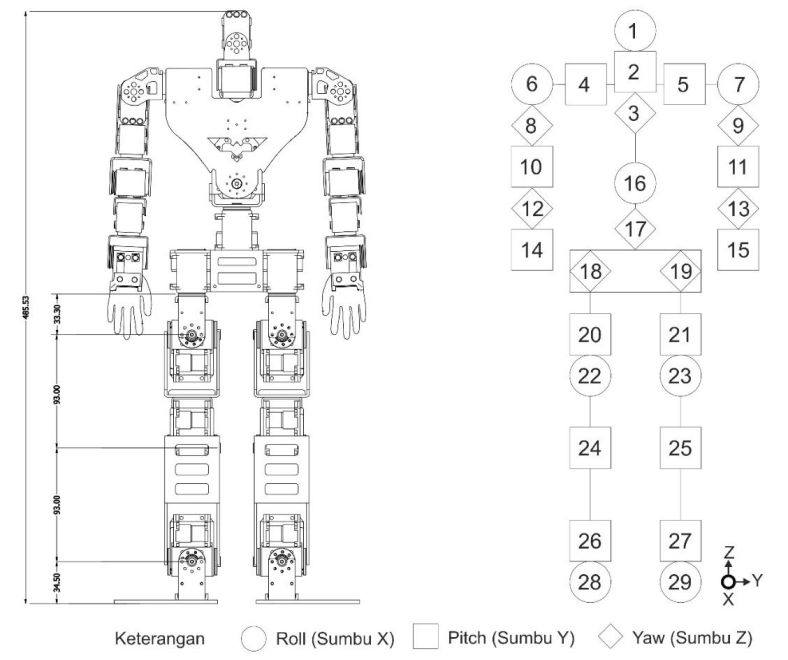
\includegraphics[width=0.35\textwidth]{gambar/Desain_Mekanik.png}
      \caption{Desain Mekanik Robot dan Penamaan ID Servo}
      \label{fig:Desain_Mekanik}
    \end{figure}

    \item Sistem Elektronik
    \label{subsec:sistemelektronik}

    \hspace*{1em} Sistem perangkat keras (hardware) dalam penelitian ini dijelaskan melalui diagram blok yang ditunjukkan pada Gambar \ref{fig:Diagram_Elektronik}. Sistem ini menggunakan sistem tertanam yang terdiri dari mikrokontroler ESP32 dan ESP32-C3. Sistem tertanam dipilih karena robot yang dikembangkan dalam penelitian ini merupakan pengembangan dari penelitian sebelumnya yang dilakukan oleh Fahd (2018)\cite{fahd}. 

    \begin{figure} [h] \centering
      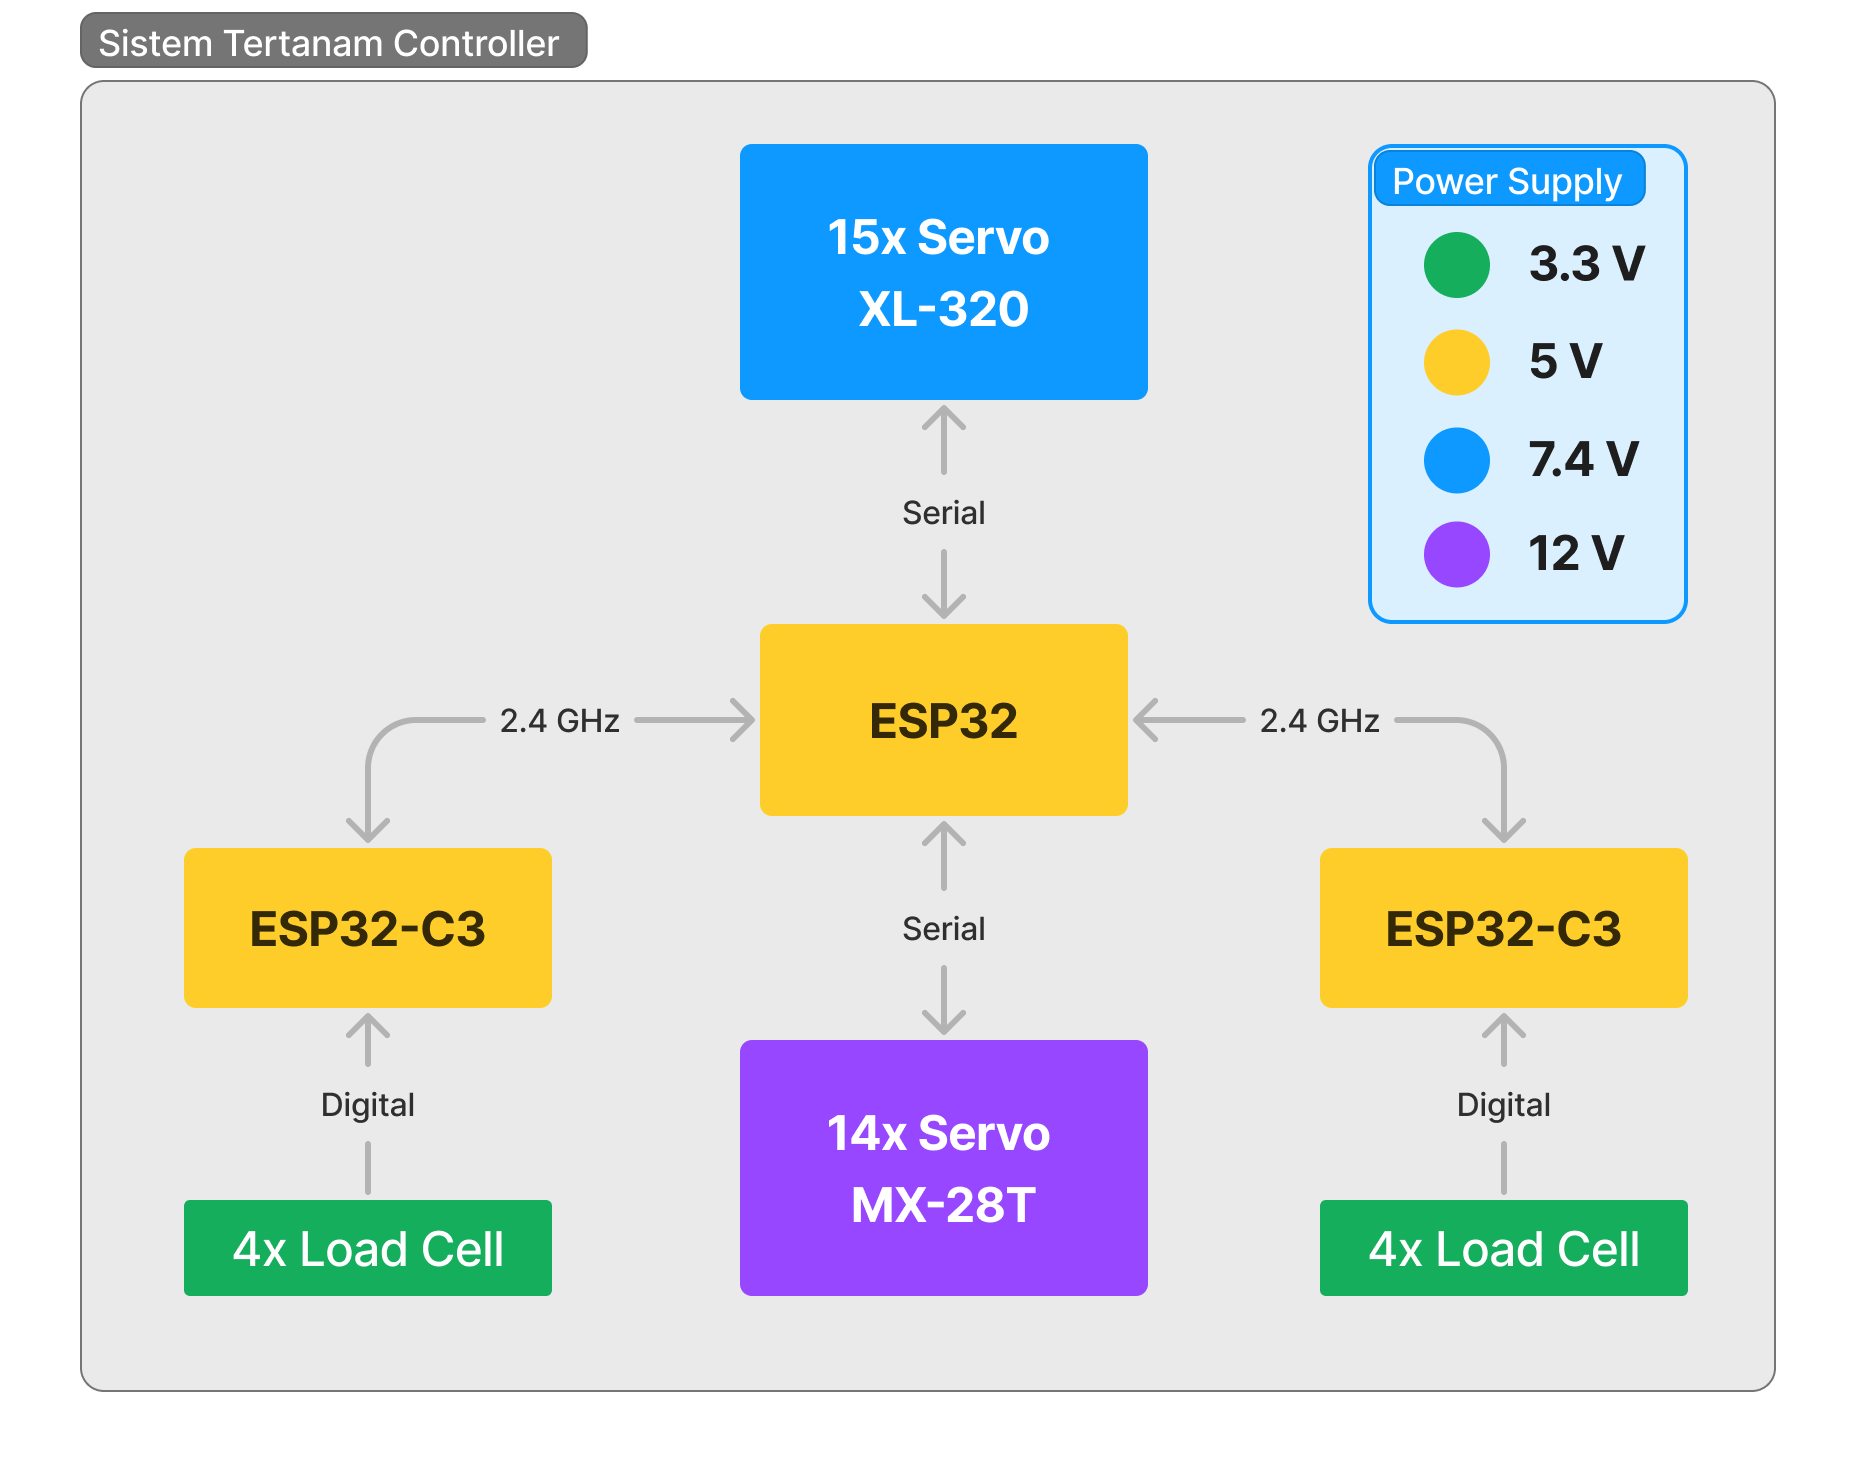
\includegraphics[width=0.4\textwidth]{gambar/Diagram_Elektronik.png}
      \caption{Diagram Elektronik dan Komunikasi Antar Komponen}
      \label{fig:Diagram_Elektronik}
    \end{figure}

    \hspace*{1em} ESP32-C3, digunakan untuk pengambilan data dari load cell dan mengirimkannya ke ESP32. ESP32-C3 memiliki kemampuan Wi-Fi yang sama dengan ESP32, sehingga memungkinkan komunikasi nirkabel antara dua mikrokontroler. ESP32-C3 juga memiliki dimensi yang lebih kecil, sehingga lebih mudah ditempatkan pada kaki robot.

    \item Desain Telapak Kaki Robot
    \label{subsec:desainsistemloadcell}

    \hspace*{1em} Setiap telapak kaki robot dilengkapi dengan 4 \emph{load cell} yang terpasang di ujung-ujung kaki. Masing-masing \emph{load cell} mendeteksi tekanan, sehingga memungkinkan sistem untuk menentukan posisi pusat tekanan pada telapak kaki robot. Desain telapak kaki robot dapat dilihat pada Gambar \ref{fig:Desain_Kaki}.
    
    \begin{figure} [h] \centering
      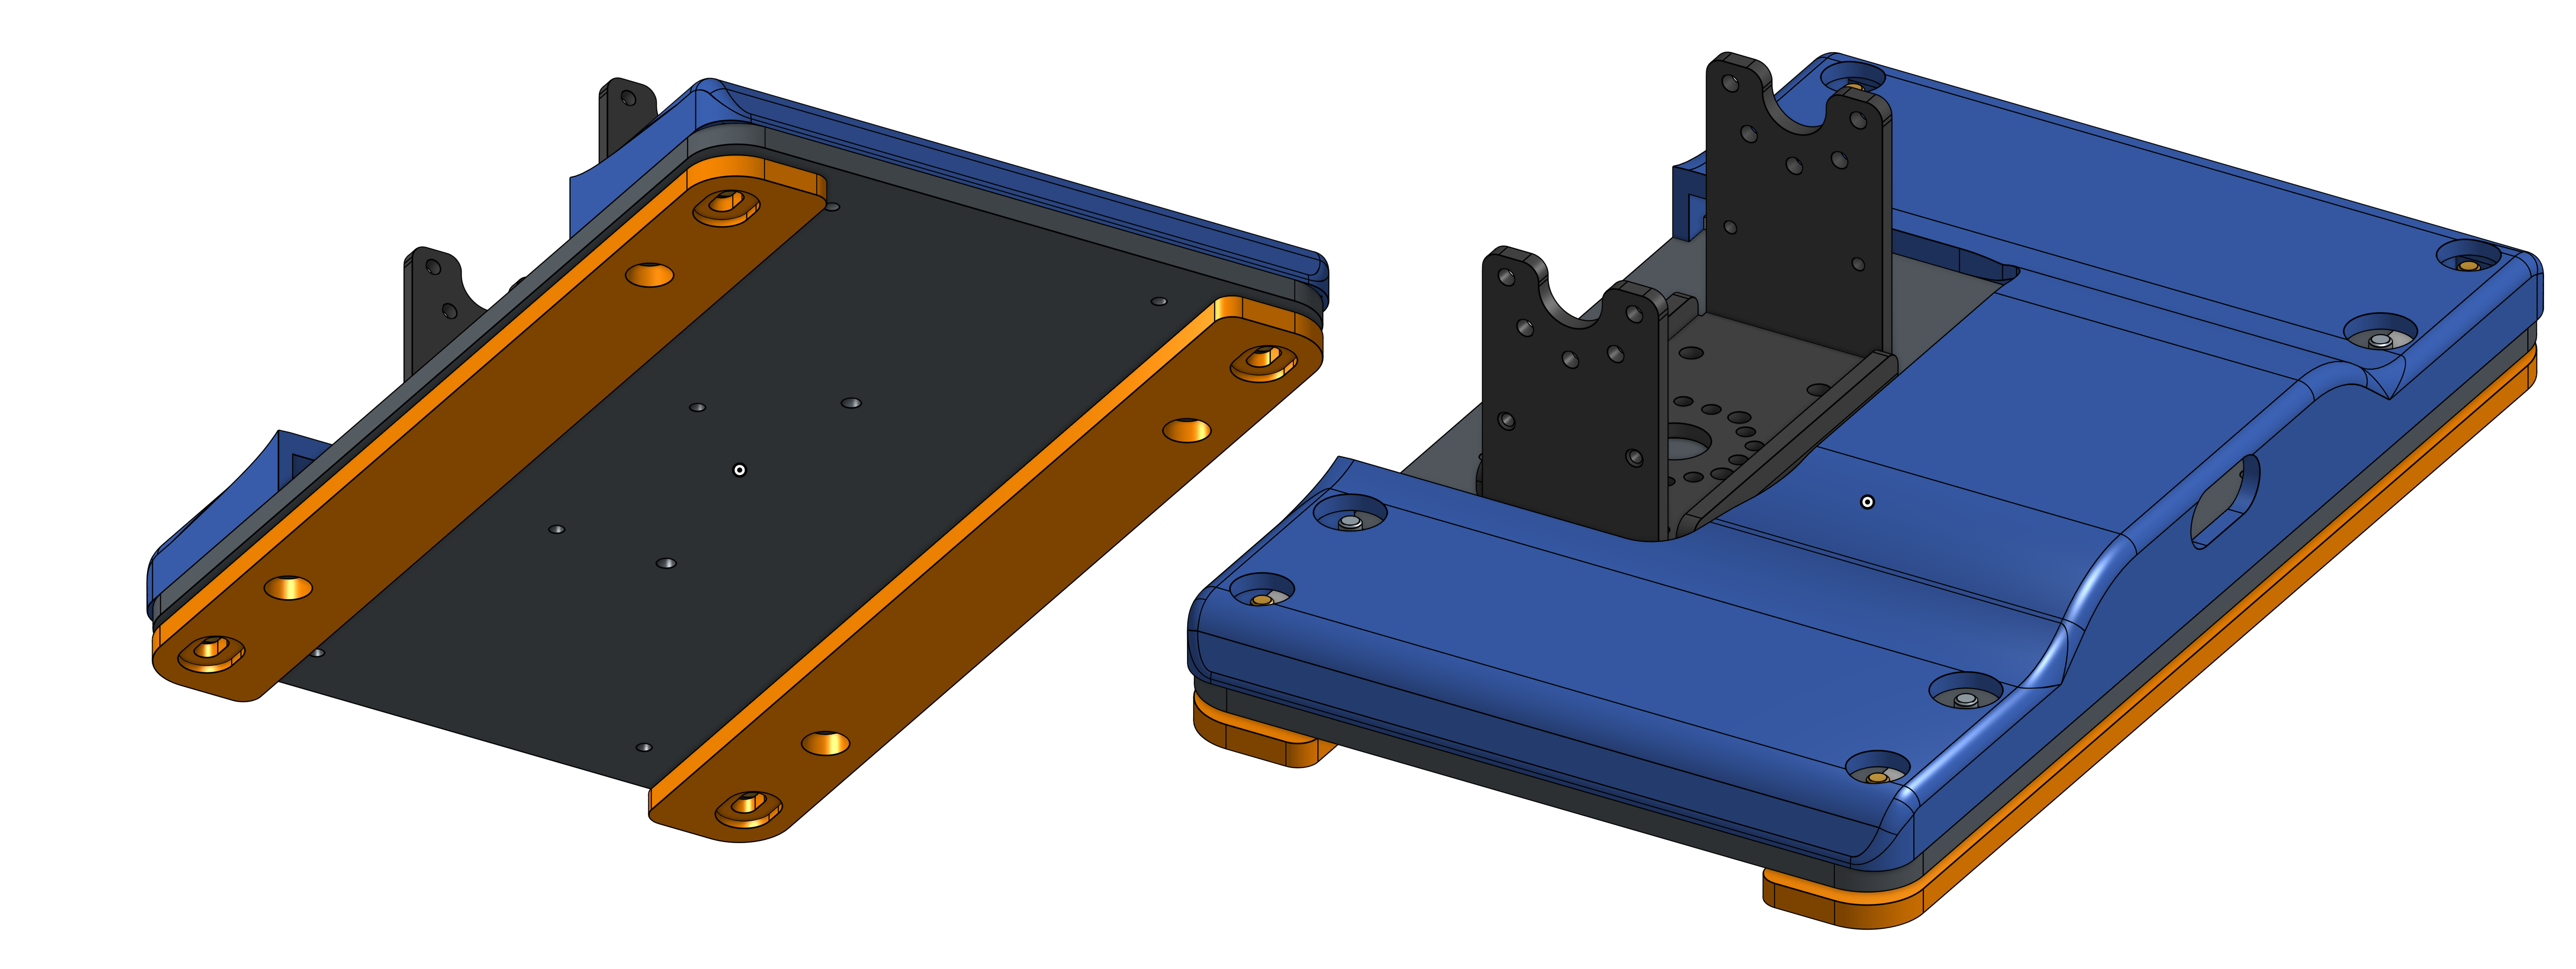
\includegraphics[width=0.4\textwidth]{gambar/Desain_Kaki.png}
      \caption{Desain Telapak Kaki Robot secara Keseluruhan}
      \label{fig:Desain_Kaki}
    \end{figure}

    \hspace*{1em} Pada Gambar \ref{fig:Desain_Kaki}, terlihat bahwa setiap \emph{load cell} ditempatkan pada ujung kaki robot. \emph{Load cell} tersebut terhubung ke mikrokontroler yang terletak di dalam kaki robot. Pada bagian elektronik, telah diberikan penutup berupa \textit{closure} yang terbuat dari 3D print untuk melindungi komponen dari kerusakan. Pada bagian mekanis, sensor \emph{load cell} dilengkapi dengan \textit{pad} yang berfungsi sebagai penekan sensor \emph{load cell} ke permukaan dan juga anti slip agar tidak mudah tergelincir.  

    \item Kongurasi Koefisien \emph{Load Cell}
    \label{subsec:konfigurasikoefisien}

    \hspace*{1em} Sebelum \emph{load cell} dapat digunakan, perlu dilakukan kalibrasi untuk mengukur koefisien \emph{load cell} dengan mengatur parameter seperti nilai koefisien \textit{scaling} dan \textit{offset}. Untuk mempermudah pengaturan, dibuatkan aplikasi konfigurasi dengan antarmuka pengguna grafis (GUI) yang mudah digunakan dan dapat diakses melalui browser. GUI ini memiliki control menu untuk mengakses fungsi dan pengaturan, serta menampilkan titik pusat tekanan yang memberikan visualisasi dampak perubahan parameter terhadap sistem. Gambar \ref{fig:Preview_Aplikasi} menunjukkan tampilan aplikasi konfigurasi, termasuk control menu dan tampilan titik pusat tekanan. Aplikasi ini akan menyimpan data konfigurasi ke dalam memori EEPROM mikrokontroler, sehingga data tetap tersimpan meskipun mikrokontroler dimatikan.

    \begin{figure} [h] \centering
      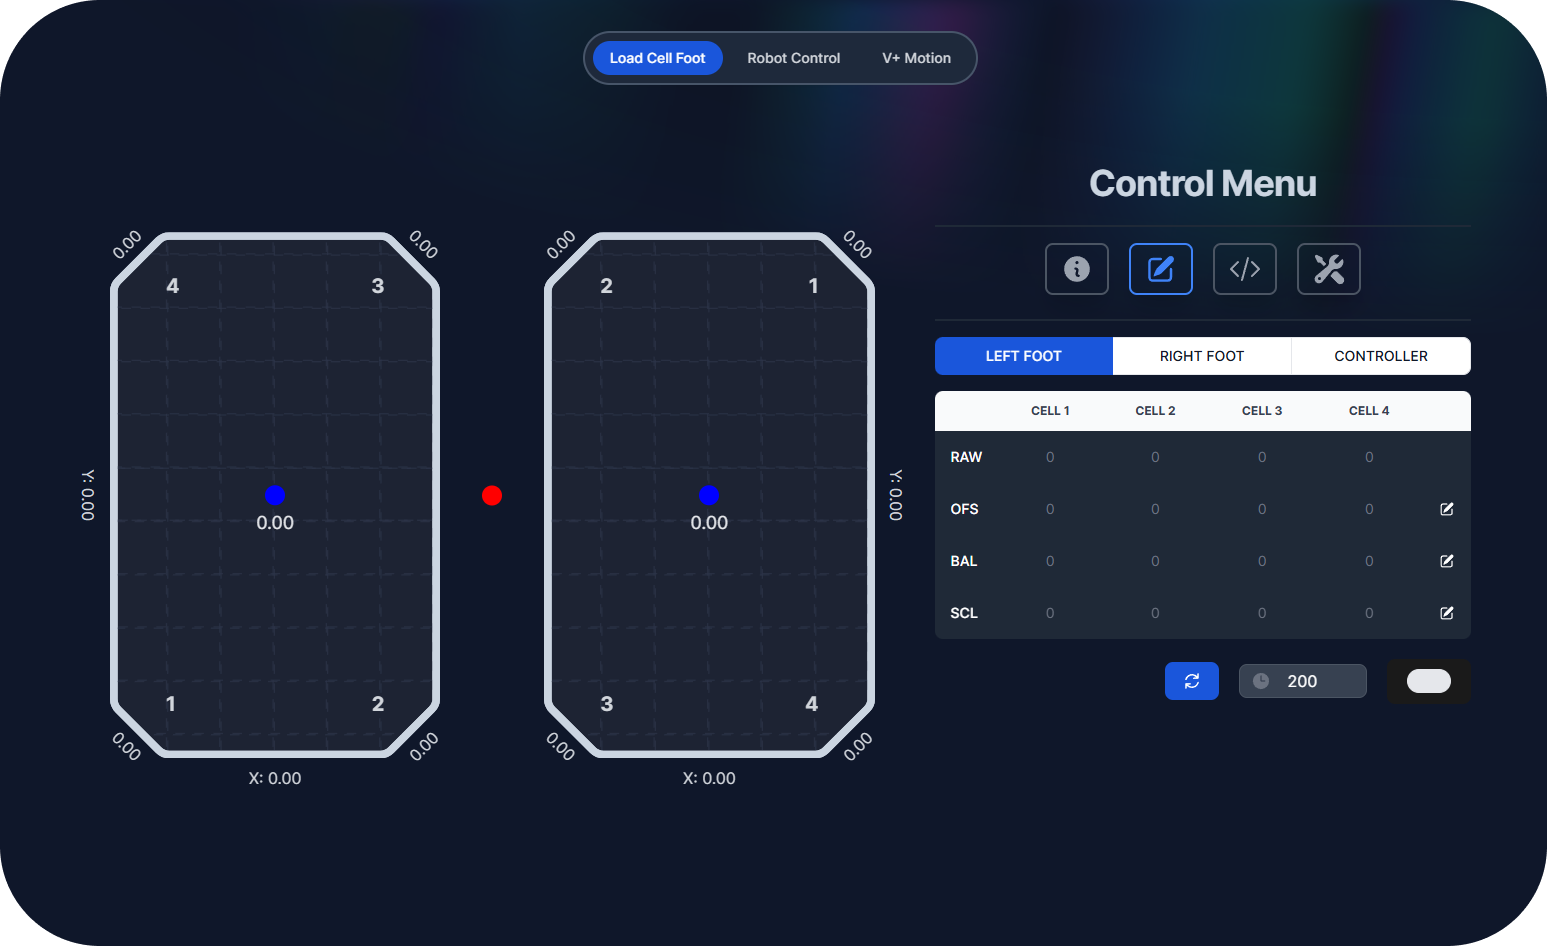
\includegraphics[width=0.4\textwidth]{gambar/preview_aplikasi.png}
      \caption{Aplikasi yang Digunakan untuk Konfigurasi \emph{Load Cell}}
      \label{fig:Preview_Aplikasi}
    \end{figure}

    \item Perhitungan Pusat Tekanan terhadap Robot
    \label{subsec:perhitunganpusattekanan}

    \hspace*{1em} Pusat tekanan pada robot dihitung dengan menggabungkan data dari kedua kaki robot. Mikrokontroler utama akan berkomunikasi dengan mikrokontroler pada kaki kiri dan kaki kanan untuk mendapatkan data pusat tekanan dan total tekanan. Data tersebut kemudian digunakan untuk mendapatkan posisi pusat tekanan terhadap robot. Perhitungan posisi pusat tekanan pada robot dilakukan seperti pada persamaan \ref{eq:Total_Force_Robot}, \ref{eq:COP_X_Robot}, dan \ref{eq:COP_Y_Robot}. 
    
    \begin{figure} [h] \centering
      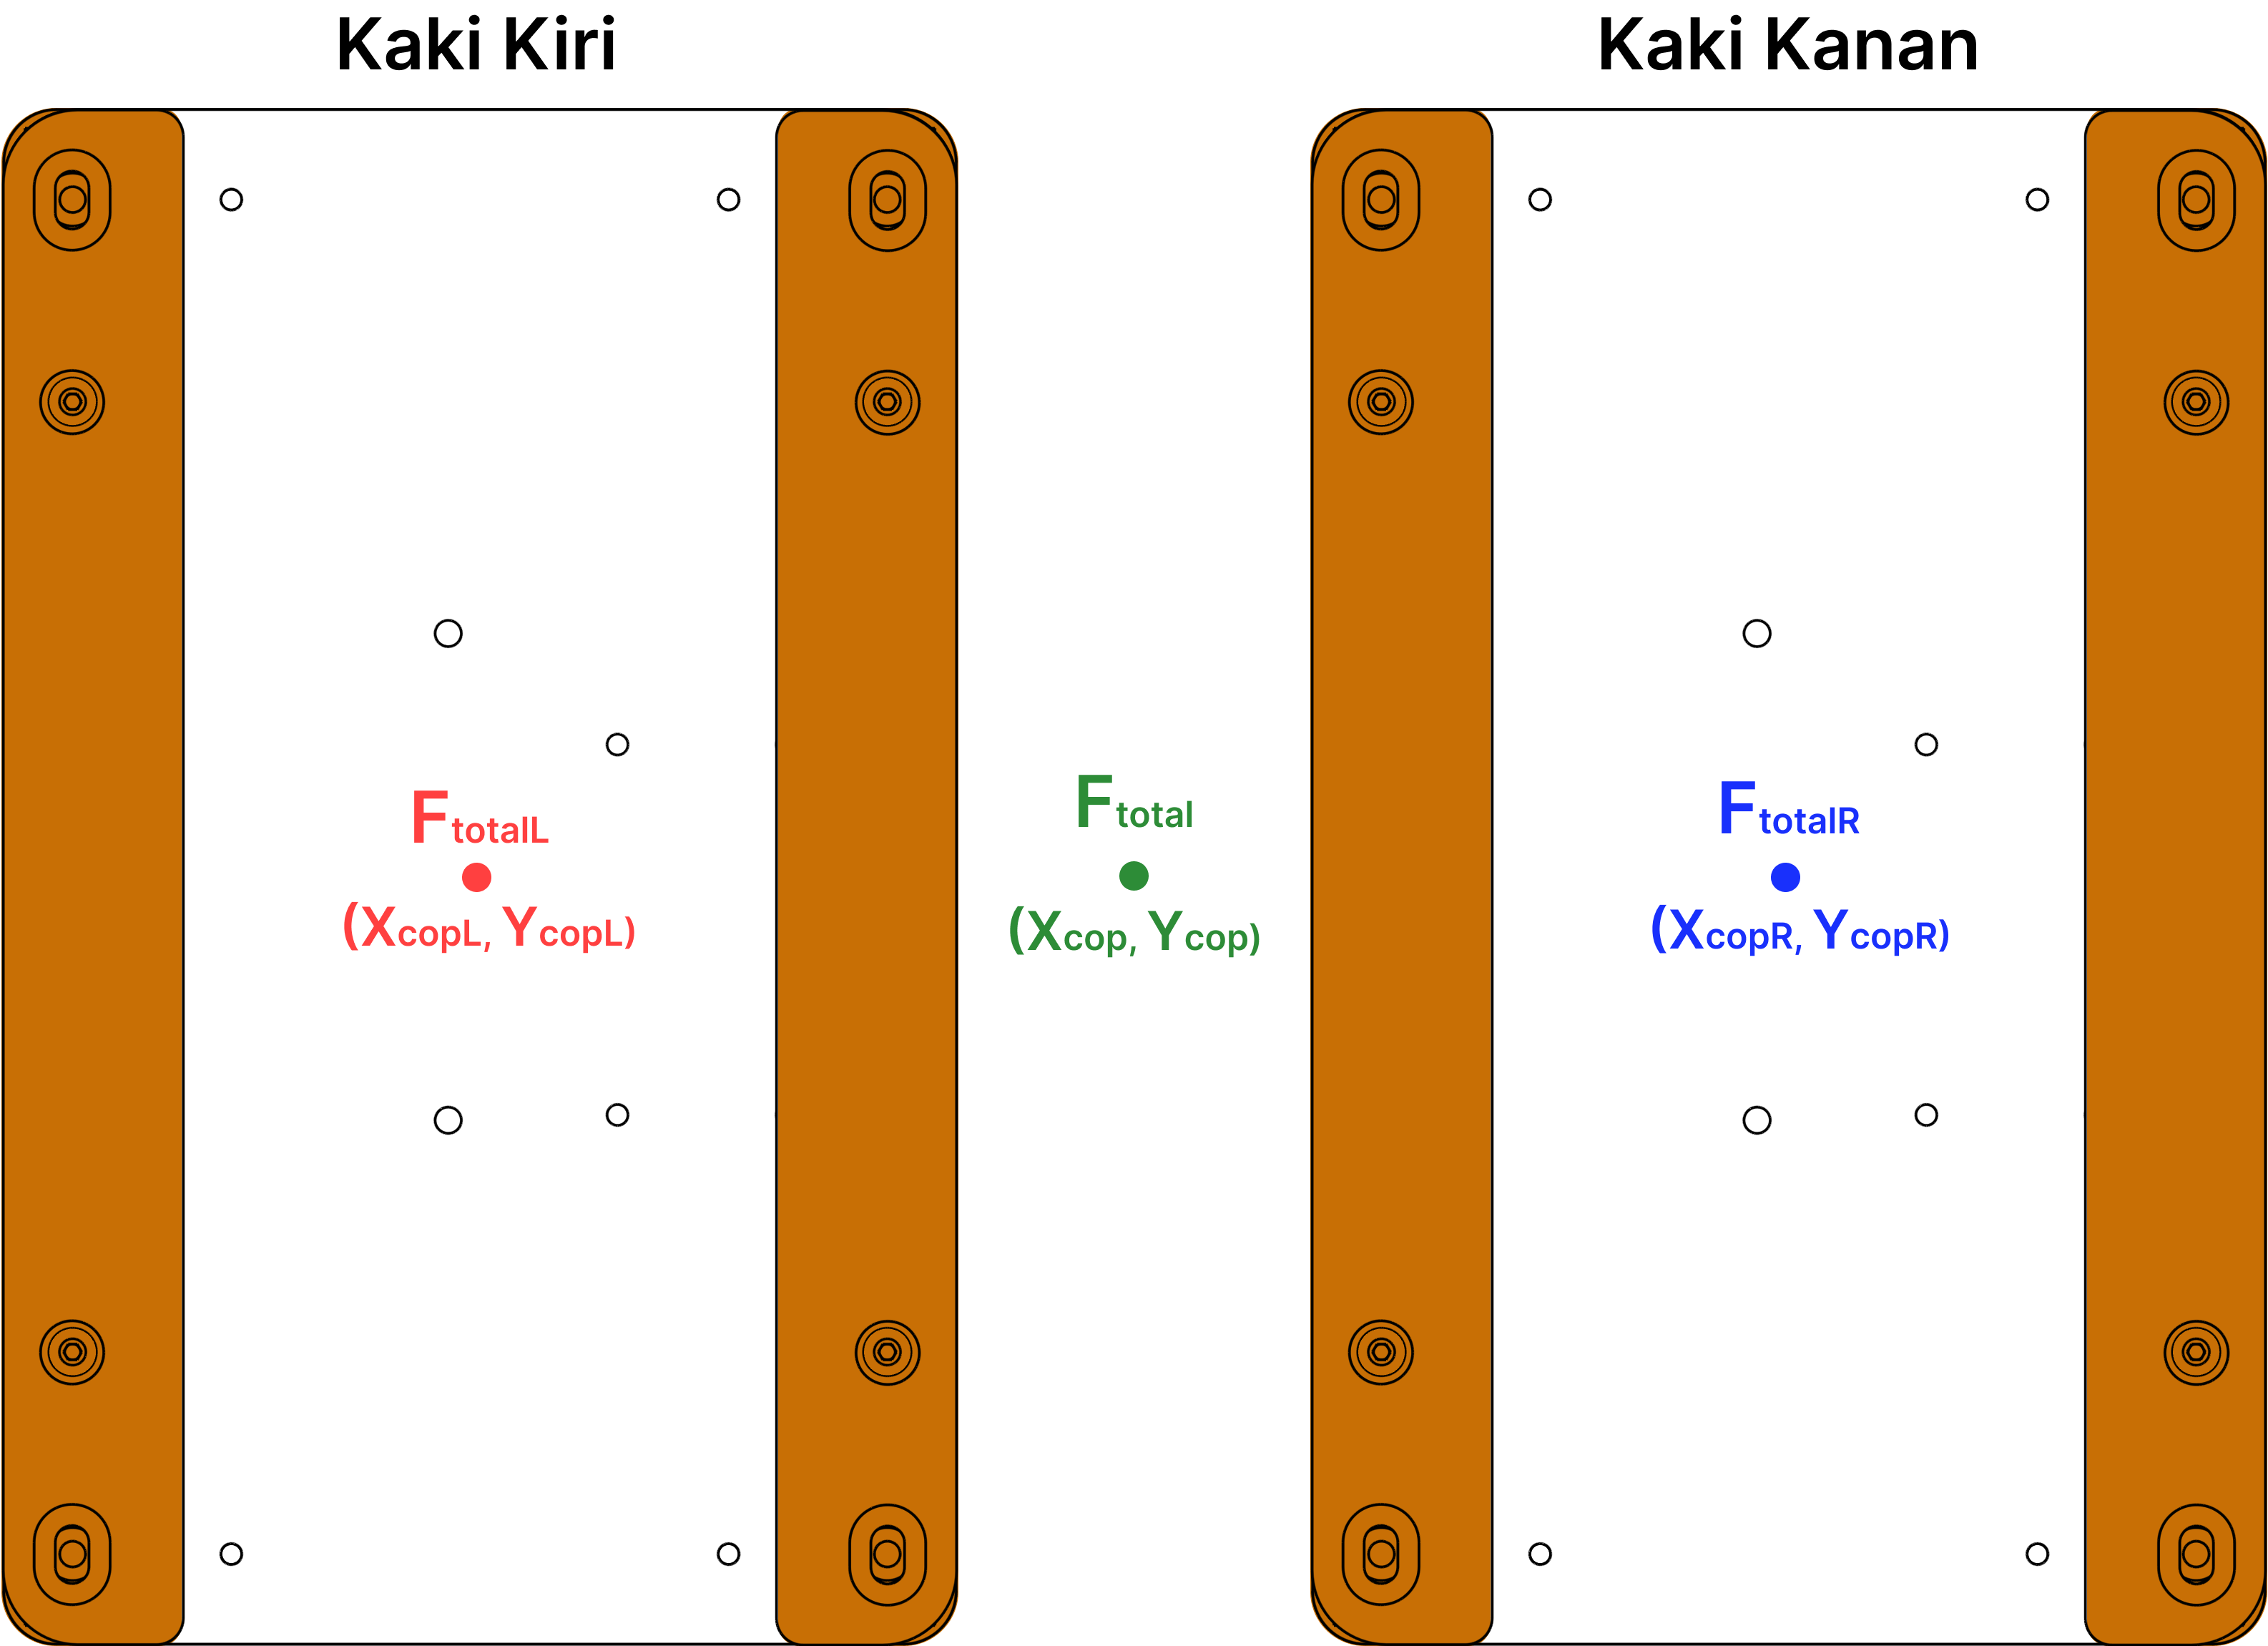
\includegraphics[width=0.4\textwidth]{gambar/COP_Robot.png}
      \caption{Pusat Tekanan pada Robot (Hijau), Pusat Tekanan pada Kaki Kiri (Merah), dan Pusat Tekanan pada Kaki Kanan (Biru)}
      \label{fig:COP_Robot}
    \end{figure}

    \begin{equation}
      F_{\mathrm{total}} = F_{\mathrm{totalL}} + F_{\mathrm{totalR}}
      \label{eq:Total_Force_Robot}
    \end{equation}

    \begin{equation}
      X_{\mathrm{cop}} = \frac{F_{\mathrm{totalL}} \cdot X_{\mathrm{copL}} + F_{\mathrm{totalR}} \cdot X_{\mathrm{copR}}}{F_{\mathrm{total}}}
      \label{eq:COP_X_Robot}
    \end{equation}

    \begin{equation}
      Y_{\mathrm{cop}} = \frac{F_{\mathrm{totalL}} \cdot Y_{\mathrm{copL}} + F_{\mathrm{totalR}} \cdot Y_{\mathrm{copR}}}{F_{\mathrm{total}}}
      \label{eq:COP_Y_Robot}
    \end{equation}

    \hspace*{1em} Data pusat tekanan pada penelitian ini akan menggunakan skala. Sesuai dengan Gambar \ref{fig:COP_Robot}, sumbu Y memiliki skala dari -1 hingga 1. Batas atas diwakili oleh nilai 1, sedangkan batas bawah diwakili oleh nilai -1. Sedangkan pada sumbu X memiliki skala dari -2 hingga 2, dengan batas kanan diwakili oleh nilai 2 dan batas kiri diwakili oleh nilai -2. Untuk sumbu X, ketika berat robot bertumpu pada salah satu kaki, nilai pusat tekanan akan bernilai positif atau negatif tergantung pada posisi kaki yang bertumpu. Ketika robot diangkat, nilai pusat tekanan akan berada pada titik (0,0) yang berada di tengah-tengah telapak kaki. 

    \item Algoritma Sistem Kontrol PID
    \label{subsec:algoritmakontrolpid}

    \hspace*{1em} Pada penelitian ini, terdapat dua kontrol PID, yaitu kontrol PID Pitch dan kontrol PID Roll. Pada kontrol PID Pitch, input berupa nilai posisi pusat tekanan pada sumbu Y. Sedangkan pada kontrol PID Roll, input berupa nilai posisi pusat tekanan pada sumbu X. Untuk setpoint kontrol PID Pitch dan Roll, digunakan nilai yang sudah ditemukan pada pengambilan data input pusat tekanan sebelumnya. Nilai error diperoleh dari selisih antara posisi pusat tekanan saat ini dengan setpoint seperti pada Persamaan \ref{eq:Error_PID} dan koreksi PID dihitung dengan Persamaan \ref{eq:Koreksi_PID}.

    \begin{equation}
      \mathrm{e} = COP_{\mathrm{error}} = COP_{\mathrm{set}} - COP_{\mathrm{input}}
      \label{eq:Error_PID}
    \end{equation}

    \begin{equation}
      \mathrm{Koreksi} = \mathrm{Kp} \cdot \mathrm{e} + \mathrm{Ki} \cdot \int \mathrm{e} + \mathrm{Kd} \cdot \frac{\mathrm{de}}{\mathrm{dt}}
      \label{eq:Koreksi_PID}
    \end{equation}

    \begin{figure} [h] \centering
      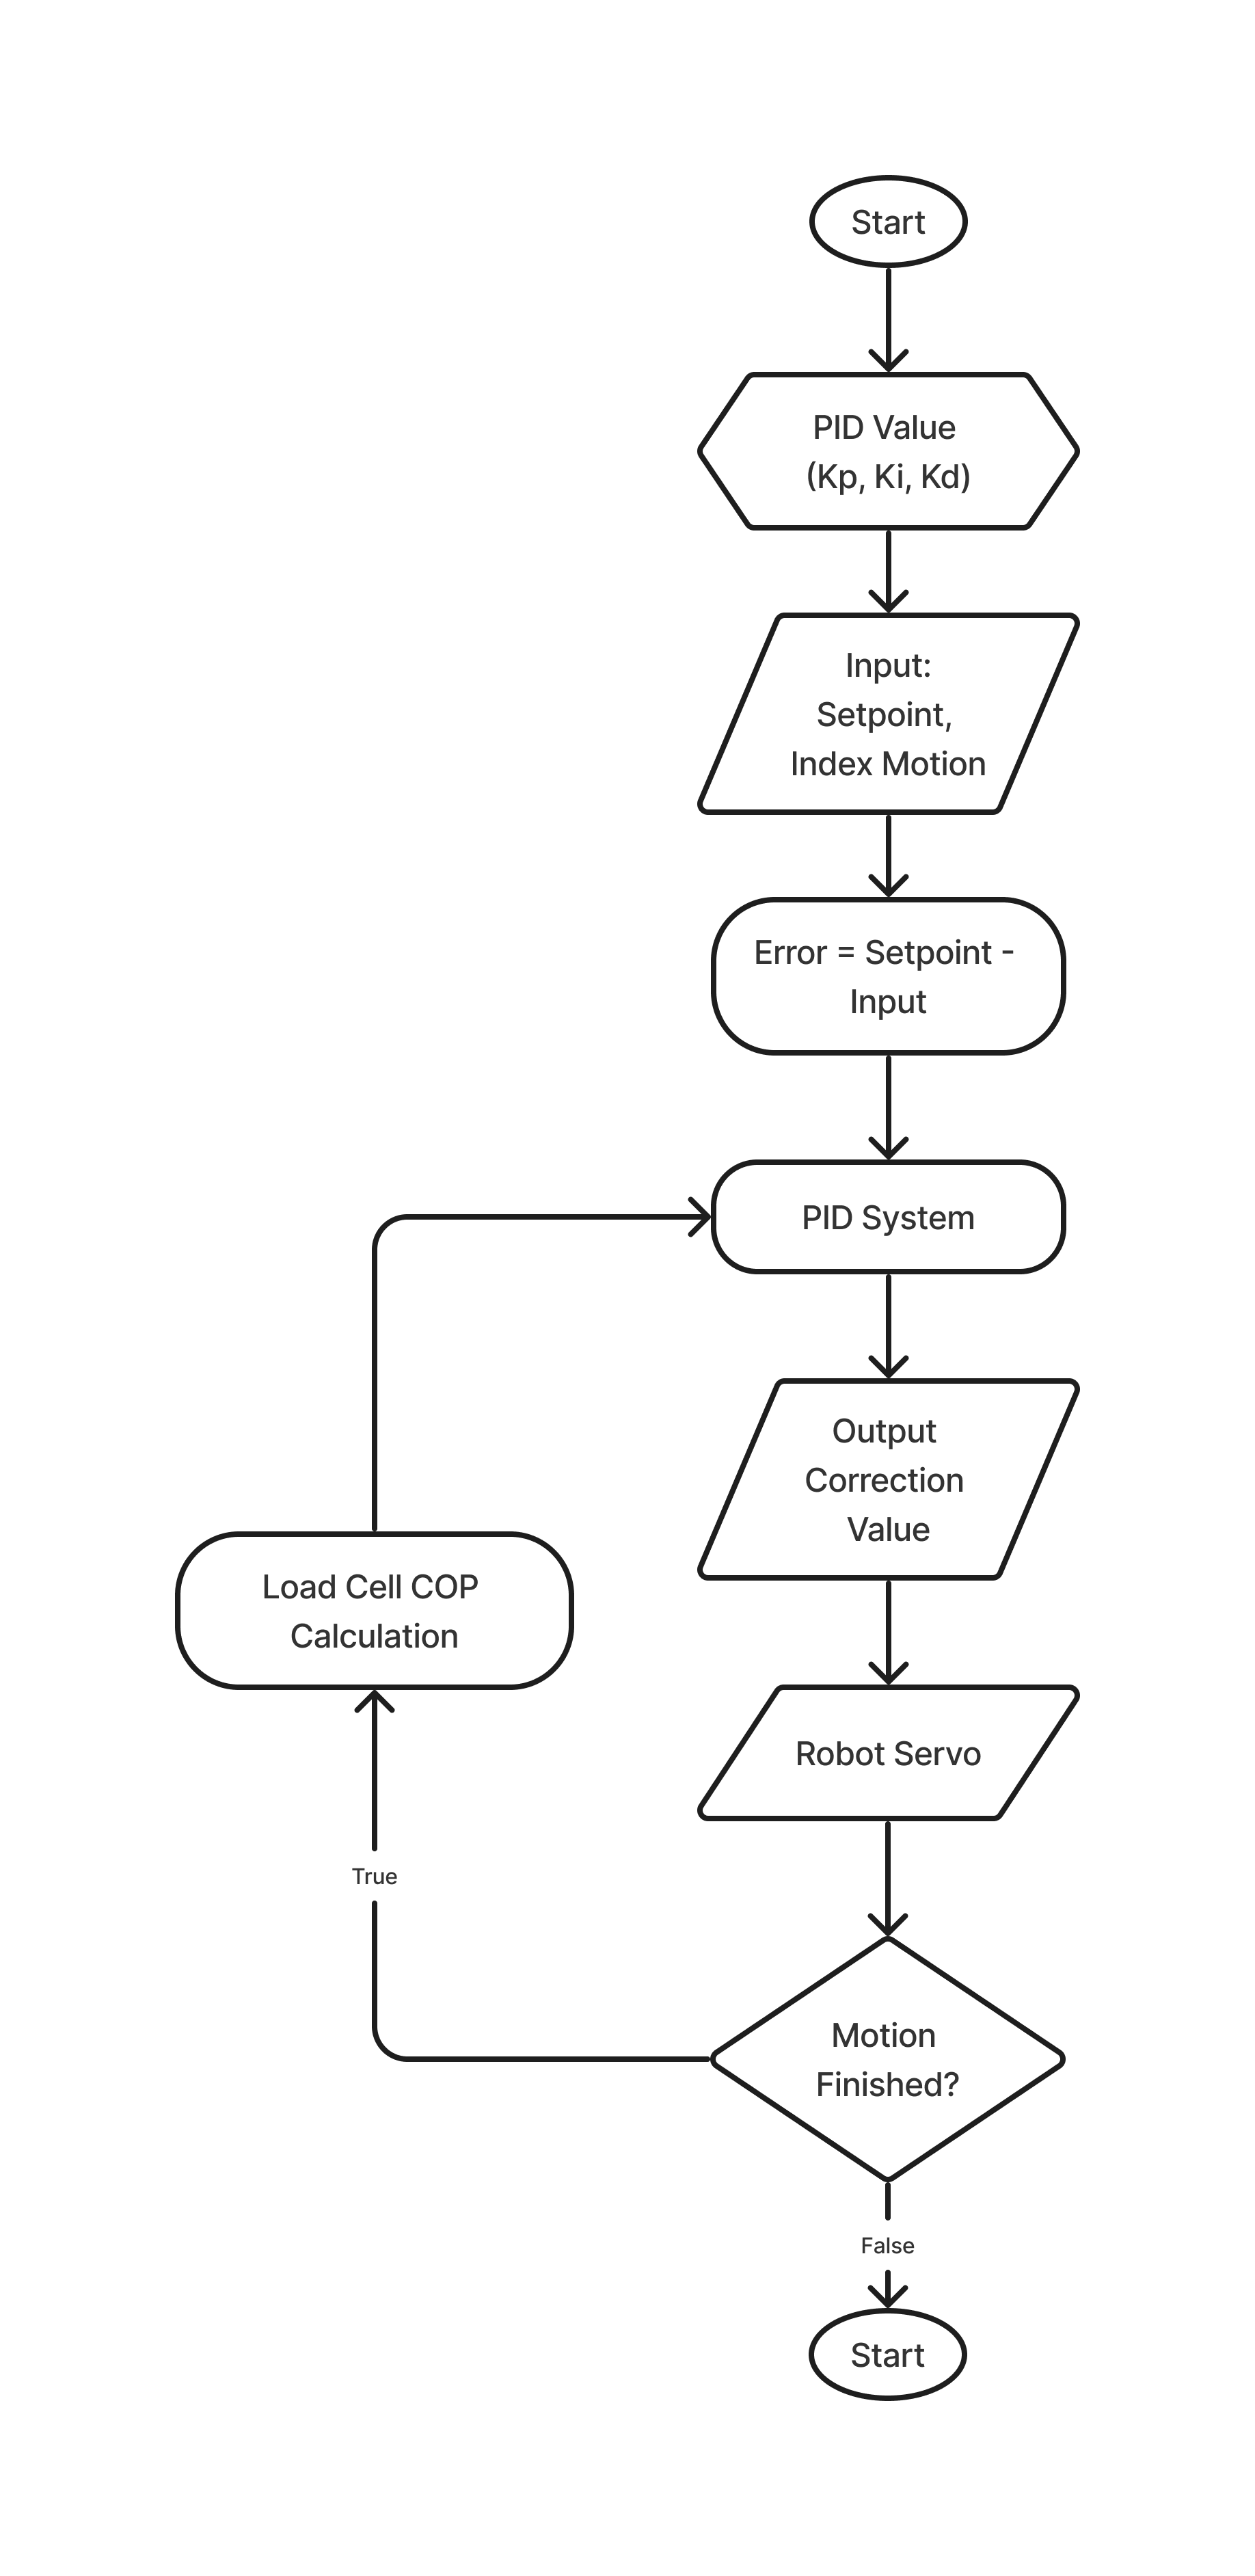
\includegraphics[width=0.38\textwidth]{gambar/Flow_Kontrol.png}
      \caption{Diagram Alir Sistem Kontrol PID Ketika \textit{Motion} Robot Berjalan}
      \label{fig:Flow_Kontrol}
    \end{figure}
    
    \hspace*{1em} Pada flowchart Gambar \ref{fig:Flow_Kontrol}, ditunjukkan tahapan respon sistem terhadap \textit{error} yang disebabkan oleh perbedaan antara posisi pusat tekanan yang diinginkan dan yang sebenarnya. Pertama, nilai PID diatur sesuai karakteristik sistem, kemudian setpoint diatur sesuai posisi pusat tekanan yang diinginkan. \textit{Error} dihitung dengan mengurangkan nilai setpoint dari nilai input menggunakan persamaan \ref{eq:Error_PID}. Nilai \textit{error} ini digunakan untuk menghitung koreksi menggunakan persamaan \ref{eq:Koreksi_PID}, yang kemudian digunakan untuk mengatur posisi servo sebagai kompensasi. Robot akan melakukan gerakan untuk menjaga keseimbangan berdasarkan koreksi yang dihasilkan oleh kontrol PID, yang berjalan terus menerus hingga \textit{motion} robot selesai.

    \begin{figure} [h] \centering
      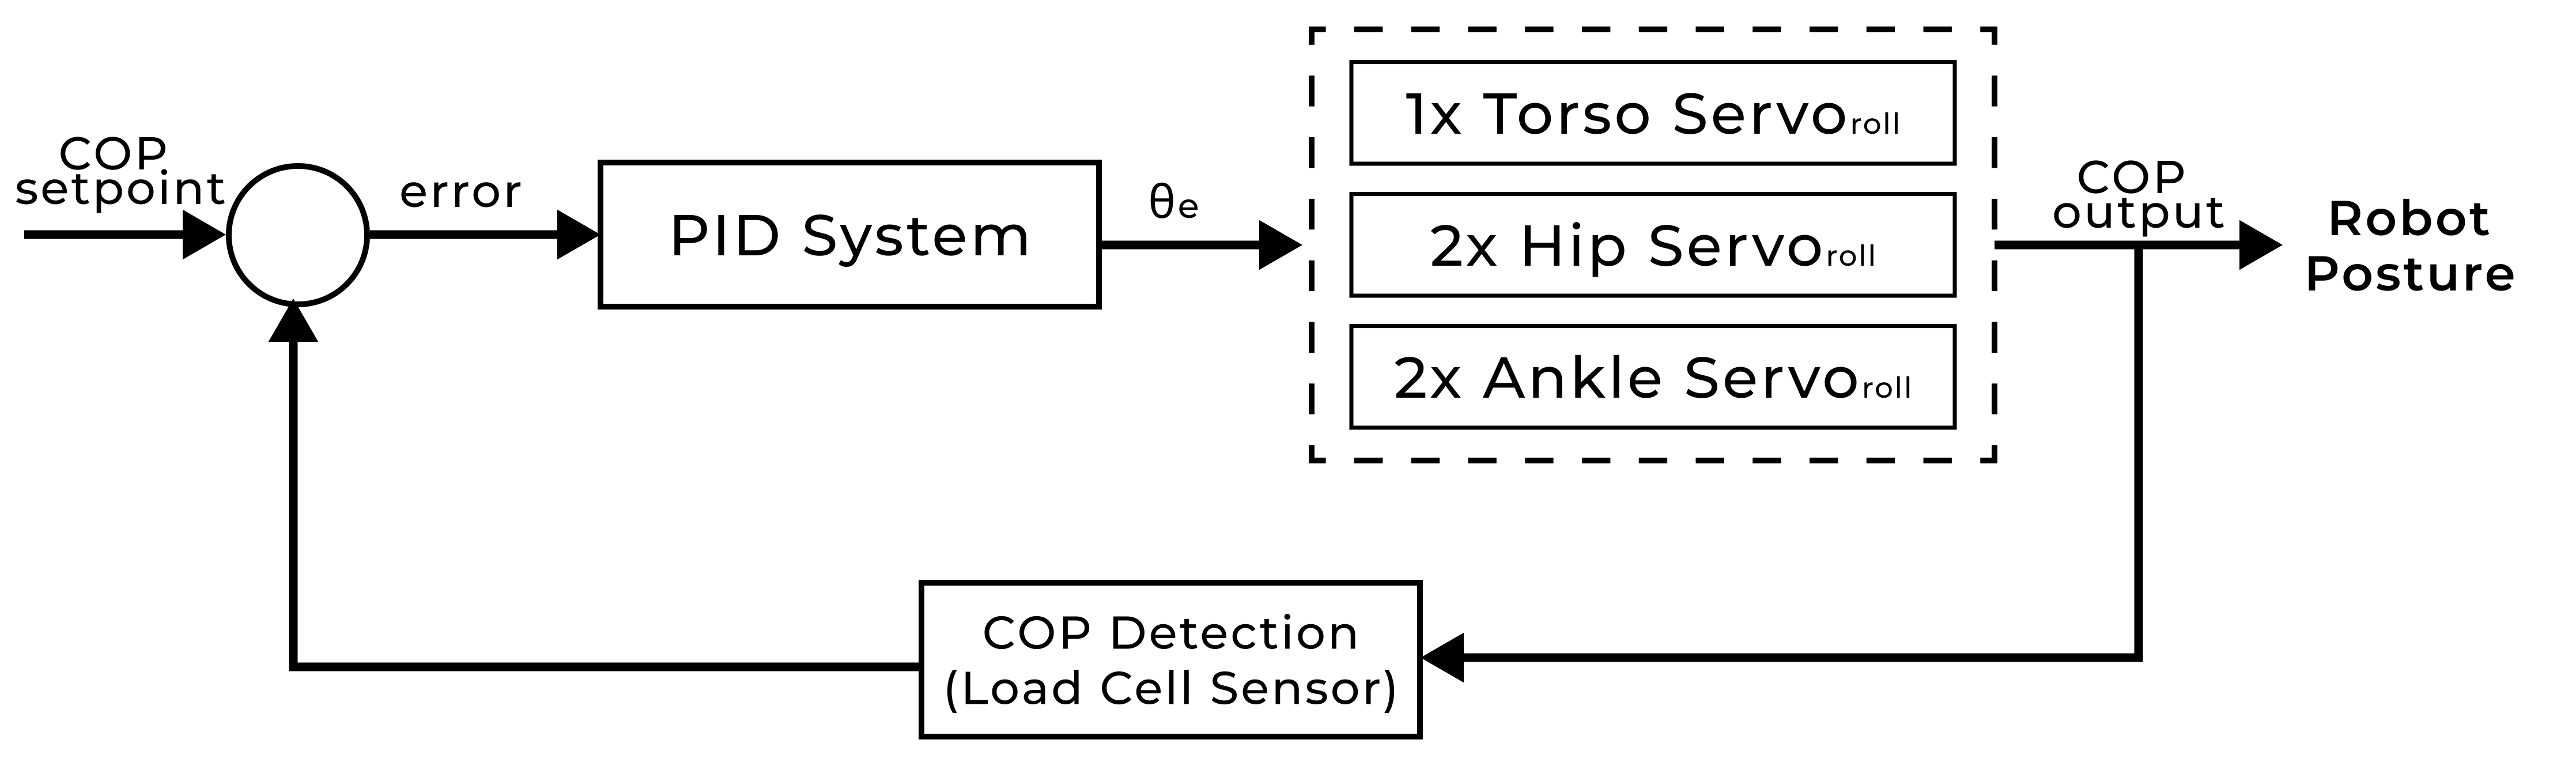
\includegraphics[width=0.4\textwidth]{gambar/pid_diagram.png}
      \caption{Diagram Sistem Kontrol PID}
      \label{fig:Control_System}
    \end{figure}

    \hspace*{1em}  Gambar \ref{fig:Control_System} menunjukkan diagram sistem kontrol yang terdiri dari tiga blok utama: blok kontrol PID, blok servo sebagai kompensasi, dan blok pusat tekanan. Blok kontrol PID menghitung nilai koreksi berdasarkan \textit{error} antara posisi pusat tekanan yang diinginkan dan yang sebenarnya. Nilai koreksi ini digunakan untuk mengatur posisi servo pada blok servo sebagai kompensasi. Blok pusat tekanan menghitung posisi pusat tekanan pada telapak kaki robot dan menyediakan data ini sebagai input pada kontrol PID.

    \item Pengaturan Servo sebagai Kompensasi
    \label{subsec:servosettings}

    \hspace*{1em} Pada penelitian ini, servo yang digunakan untuk menjaga keseimbangan adalah servo yang mengatur posisi \textit{roll} robot. Servo tersebut terletak pada \textit{torso}, \textit{hip}, dan \textit{ankle}. Servo pada \textit{torso}, \textit{hip}, dan\textit{ankle}. Dengan mengatur beberapa sudut servo, robot dapat melakukan penyesuaian yang diperlukan untuk mempertahankan keseimbangan saat bergerak atau berdiri di permukaan yang tidak rata. Terdapat lima servo yang digunakan yang terdiri dari satu servo pada \textit{torso} (ID 1), dua servo pada masing-masing \textit{hip} (ID 4 dan ID 5), dan dua servo pada masing-masing \textit{hip} (ID 13 dan ID 14). Pengaturan servo sebagai kompensasi dapat dilihat pada Gambar \ref{fig:Controlled_Servo}, ditunjukkan oleh servo yang diwarnai biru.

    \begin{figure} [h] \centering
      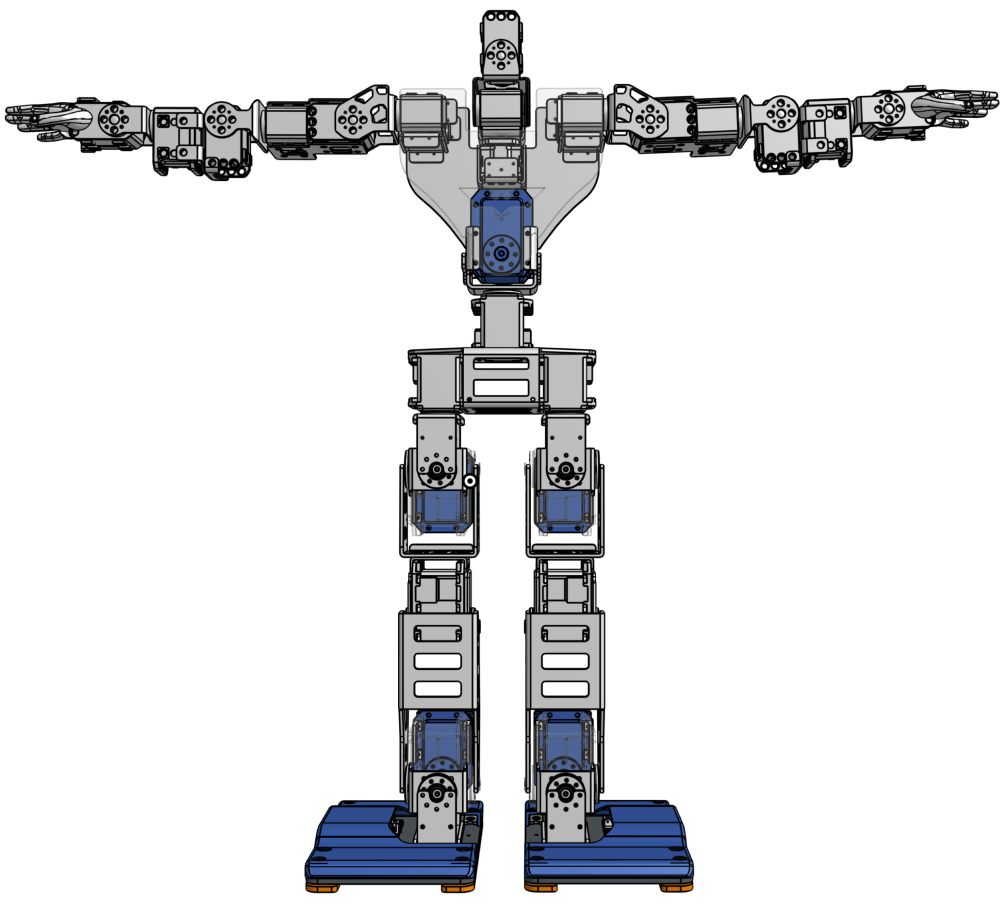
\includegraphics[width=0.4\textwidth]{gambar/controlled_servo.png}
      \caption{Pengaturan Servo sebagai Kompensasi Ditunjukkan dengan Warna Biru}
      \label{fig:Controlled_Servo}
    \end{figure}

    \hspace*{1em} 
\end{enumerate}